%%%%%%%%%%%%%%%%%%%%%%%%%%%%%%%%%%%%%%%%%%%%%%%%%%%
%% Capítulo 4: Sistemas de funciones iteradas
%%%%%%%%%%%%%%%%%%%%%%%%%%%%%%%%%%%%%%%%%%%%%%%%%%%

Como venimos viendo ya en los dos últimos capítulos, la iteración es una poderosa herramienta en la generación de imágenes fractales. Sin embargo, hasta ahora siempre nos estamos basando en buscar convergencia y velocidad de convergencia de sucesiones de iteradas de funciones complejas, las cuales evalúan un número complejo $z\in\C$ para devolver otro número complejo $f(z)\in\C$. Si recuperamos la identificación $z=x+y\cdot i\simeq (x,y)\in\R^2$ podemos ver las funciones complejas como campos vectoriales de $\R^2$, y si en lugar de aplicar una función a un único punto la aplicamos a un conjunto de puntos llegamos a la base de los \textit{Sistemas de Funciones Iteradas}, en adelante SFI. 

La matemática que explica los SFI se puede encontrar en el clásico libro \textit{Fractals Everywhere}\cite{Barnsley} de \textit{Michael Barnsley}. Por su parte, la geometría fractal nació en 1977 con la publicación de \textit{The fractal geometry of nature}\cite{alma991007242979704990} por parte de \textit{Benoit Mandelbrot}. En general, gracias a la geometría fractal y ayudándonos de los SFI podemos recrear resultados de imágenes y objetos con un nivel de detalle que la geometría euclídea no puede conseguir. Sin embargo, el problema inverso también es interesante: ¿es posible, a partir de un objeto, describirlo matemáticamente mediante SFI? Este es un área de la matemática aún abierta y en la que a día de hoy se continua trabajando. Uno de los resultados más conocidos en este ámbito es el \textit{teorema del collage}, del cual hablaremos más adelante. %TODO referenciar teorema y sección

\section{Transformaciones afines en el plano euclídeo y SFI}

Si nos restringimos al plano euclídeo $\R^2$ visto como espacio afín, previo a la definición formal de SFI necesitamos unas nociones sobre transformaciones afines y maneras de representarlas, ya que estas serán las que compongan fundalmente los SFI.

\begin{definicion}[Transformación afín]
    Una transformación $w:\R^2\longrightarrow\R^2$ de la forma
    \begin{equation}
        w(x_1,x_2)=(ax_1+bx_2+e,cx_1+dx_2+f) \ \ \forall (x_1,x_2)\in\R^2
    \end{equation}
    donde las constantes $a,b,c,d,e,f$ son números reales es denominada una \textbf{transformación afín} del plano euclídeo.
\end{definicion}

Una forma equivalente de denotar $w$ matricialmente es tomando la matriz $A=\begin{pmatrix}
    a & b \\
    c & d
\end{pmatrix}\in\mathcal{M}_2(\R)$ y el vector $b=\begin{pmatrix}
    e \\
    f
\end{pmatrix}$ y expresar $w$ como:

\begin{equation}
    w(x) =
    w\begin{pmatrix}
        x_1 \\
        x_2
    \end{pmatrix} = Ax + b = \begin{pmatrix}
        a & b \\
        c & d
    \end{pmatrix}\begin{pmatrix}
        x_1 \\
        x_2
    \end{pmatrix}+\begin{pmatrix}
        e \\
        f
    \end{pmatrix} \ \ \forall \ x = \begin{pmatrix}
        x_1 \\
        x_2
    \end{pmatrix}\in\R^2.
\end{equation}

La matriz $A$ también puede ser expresada de la siguiente forma:
\begin{equation}
    A = \begin{pmatrix}
        a & b \\
        c & d
    \end{pmatrix} = \begin{pmatrix}
        r\cos\alpha & -s\sin\beta \\
        r\sin\alpha & s\cos\beta
    \end{pmatrix}
\end{equation}
donde el par $(r,\alpha)$ son las coordenadas polares de $(a,c)$ y $(s,\beta+\frac \pi 2)$ son las coordenadas polares de $(b,d)$. De esta forma, una transformación afín puede verse representada por 6 números reales $r,s,\alpha,\beta,e,f$, de forma que:
\begin{itemize}
    \item $r,s$ representan una homotecia de razón $r$ en el eje $X$ y razón $s$ en el eje $Y$.
    \item $\alpha,\beta$ denotan una rotación de $\alpha$ radianes en la componente $X$ y $\beta$ en la componente $Y$.
    \item $e,f$ simbolizan una traslación de vector $b=\begin{pmatrix} e \\ f\end{pmatrix}$.
\end{itemize}

Nótese que la transformación lineal $x\mapsto Ax$ en $\R^2$ lleva un paralelogramo con un extremo en el origen en otro paralelogramo con un extremo en el origen, como consecuencia de la linealidad de las aplicaciones \textit{escalado} y \textit{rotación}. Por lo que la transformación afín $w(x)=Ax+b$ es una composición de la aplicación lineal representada por $A$, la cual transforma el espacio relativo al origen, y de la \textit{traslación} de vector $b=\begin{pmatrix} e \\ f\end{pmatrix}$. A continuación definimos un caso concreto de transformación afín más familiar.

\begin{definicion}
    Una transformación afín de $\R^2$ $w(x)=Ax+b$, para cualquier $b\in\R^2$ se denomina \textit{similitud} si la matriz $A$ tiene alguna de las siguientes formas:
    \begin{eqnarray}
        A = \begin{pmatrix}
            r\cos\alpha & -r\sin\alpha \\
            r\sin\alpha & r\cos\alpha
        \end{pmatrix}
        , &
        A = \begin{pmatrix}
            r\cos\alpha & r\sin\alpha \\
            r\sin\alpha & -r\cos\alpha
        \end{pmatrix}
    \end{eqnarray}
    para $r\not= 0,\ \ 0\leq\alpha<2\pi$. A $r$ se le llama \textit{razón de la homotecia} o factor de escala y a $\alpha$ se le llama \textit{ángulo de rotación}.
\end{definicion}

Nótese que en caso $\alpha=\pi,\beta=0$ se consigue una reflexión respecto al eje $Y$, y viceversa.

Para aclarar todos estos conceptos en la figura \ref{fig:ejemplos-ta} podemos ver cómo actúan distintas transformaciones lineales sobre una figura simple: el polígono formado al unir los vértices $(0,0), (1,0), (1.5, 0.5), (1,1)$ y $(0,1)$. Las transformaciones lineales vienen representadas en cada caso por una sextupla $w=(r,s,\alpha,\beta,e,f)$, teniendo cada elemento el significado ya definido.

\begin{figure}[ht]
    \centering
    \begin{tabular}{cc}
      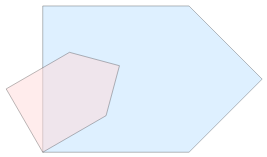
\includegraphics[scale=0.65]{./img/C4/ejemplo-ta-1.png} &   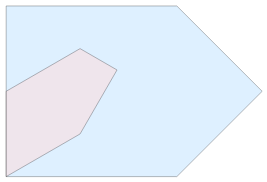
\includegraphics[scale=0.6]{./img/C4/ejemplo-ta-2.png} \\
    (a) $w=(0.5, 0.5, \frac{\pi}{6}, \frac{\pi}{6}, 0,0)$ & (b) $(0.5, 0.5, \frac{\pi}{6}, 0,0,0)$ \\[6pt]
    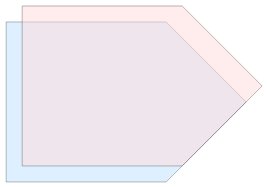
\includegraphics[scale=0.6]{./img/C4/ejemplo-ta-3.png} &   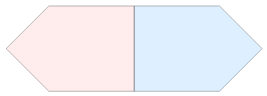
\includegraphics[scale=0.75]{./img/C4/ejemplo-ta-4.png} \\
    (c) $(1,1,0,0,0.1,0.1)$ & (d) $(1,1,\pi,0,0,0)$ \\[6pt]
    \end{tabular}
    \caption{Ejemplos de aplicaciones de transformaciones lineales}
    \label{fig:ejemplos-ta}
  \end{figure}

En el caso de (a) observamos una similitud con $r=0.5$ y $\alpha=\frac{\pi}{6}$. En (b) además de un escalado uniforme de razón $r=s=0.5$ podemos ver el efecto que tiene una rotación (no uniforme) en $X$ de razón $\alpha=\frac{\pi}{6}$. Por su parte, (c) simplemente aplica una traslación mediante el vector $b=(0.1,0.1)^t$. Por último, en (d) vemos un caso de reflexión respecto al eje $Y$.

Un último detalle para la creación de SFI es la necesidad de que las transformaciones afines utilizadas sean \textit{aplicaciones contractivas}. Procedemos por tanto a definir un SFI:

\begin{definicion}[Sistema de Funciones Iteradas]
    Un \textit{Sistema de Funciones Iteradas} se compone de un espacio métrico completo $(X,d)$ y de un conjunto finito de aplicaciones contractivas $w=\{w_i:i=1,\dots,n\}$.

    Dado un subconjunto $A\subseteq X$, la imagen de $A$ por medio de $w$ es definida como
    $$
    w(A)=\bigcup_{i=1}^n w_i(A).
    $$
\end{definicion}

En nuestro caso el espacio métrico completo es el plano euclídeo $\R^2$ y utilizaremos un conjunto finito de transformaciones lineales.

\begin{ejemplo}
    \label{ejemplo:sfi}
    Supongamos que tenemos un triángulo equilátero $T$ cuyos vértices son los puntos $(0,0),(1,0),(\frac{1}{2},\frac{\sqrt{3}}{2})$ y las transformaciones lineales
    \begin{eqnarray*}
        w_1 = \left(0.5,0.5,0,0,0,0\right) \\
        w_2 = \left(0.5,0.5,0,0,\frac 1 2,0\right) \\
        w_3 = \left(0.5,0.5,0,0,\frac 1 4,\frac{\sqrt{3}}{4}\right)
    \end{eqnarray*}
    Entonces en la imagen \ref{fig:ejemplo-sfi} podemos ver tanto $T$ como el resultado de aplicar el SFI $w$ a $T$.
    \begin{figure} [ht]
    \centering
    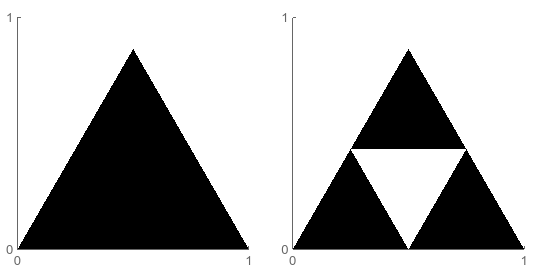
\includegraphics[scale = 0.6]{img/C4/ejemplo-sfi.png}
    \caption{Representación gráfica de $T$ y $w(T)$}
        \label{fig:ejemplo-sfi}
    \end{figure}
\end{ejemplo}

\section{Convergencia de SFI}

Probablemente el resultado de aplicar el SFI $w$ a un triángulo equilátero que vemos en el ejemplo \ref{ejemplo:sfi} le recuerde al primer paso al generar el triángulo de Sierpinski, el cual vimos en la sección \ref{subsection:triangulo-Sierpinski}. De hecho, podemos volver a aplicar $w$ a $w(T)$, a $w(w(T))$, y así sucesivamente, de forma que iterando infinitamente $w$ en $T$, el resultado final que obtenemos es efectivamente el triángulo de Sierpinski \textbf{S}, véase de nuevo la imagen \ref{fig:triangulo-Sierpinski}.

Este es sólo un ejemplo, pero a lo largo de esta sección veremos que todo SFI converge a una figura, que denominamos el atractor del sistema, independientemente de la figura inicial. Véase en la figura \ref{fig:semillas-sfi} cómo incluso tomando como semilla una figura totalmente distinta al triángulo equilátero el resultado de la iteración es el mismo. Esto es de hecho una consecuencia del Teorema del punto fijo de Banach (teorema \ref{th:punto-fijo}).

\begin{figure} [ht]
    \centering
    
\includegraphics[scale = 0.33]{img/C4/figura-X.png}
    \caption{Otra posible semilla para iterar el SFI}
        \label{fig:semilla-X}
\end{figure}

\begin{figure}[ht]
    \centering
    \begin{tabular}{cc}
      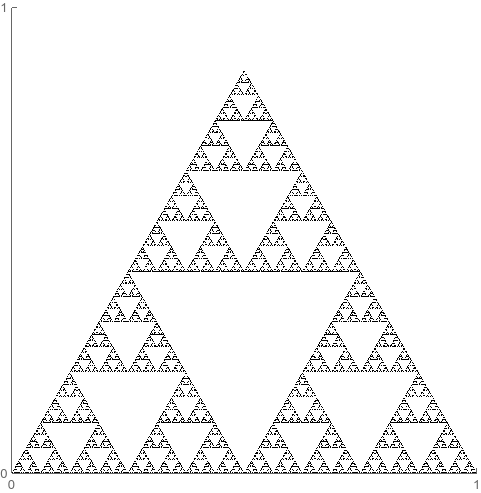
\includegraphics[scale=0.33]{./img/C4/triangulo-iterado.png} &   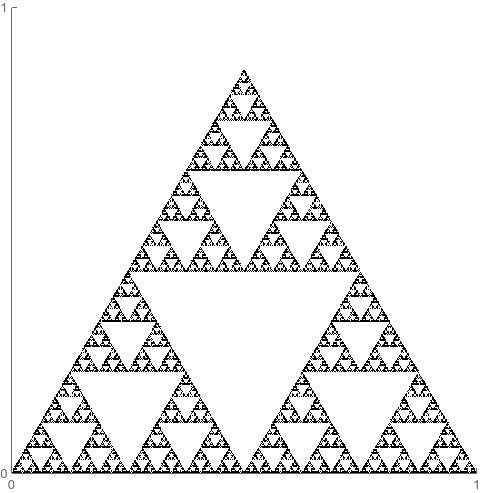
\includegraphics[scale=0.33]{./img/C4/figura-X-iterada.png} \\
    (a) Iterando un triángulo equilátero & (b) Iterando la figura \ref{fig:semilla-X} 
    \end{tabular}
    \caption{Resultado de iterar 8 veces $w$ con distintas figuras iniciales}
    \label{fig:semillas-sfi}
\end{figure}

Consideramos un espacio de Banach $(X,d)$\footnote{Recordamos que un espacio de Banach es un espacio métrico completo} y sea $\mathcal{H}(X)\subset\mathcal P (X)$ el conjunto de todos los subconjuntos compactos de $X$, el cual también se denomina \textit{espacio de fractales} de $X$. Dado un punto $x\in X$ y un subconjunto $A\in\mathcal H$ la distancia de un punto a un conjunto como
$$
d(A,B) = \inf\{d(x,b):b\in B\}=\min\{d(x,b):b\in B\},
$$
donde el ínfimo es un mínimo porque $A$ es compacto. Si tomamos dos compactos $A,B\in\mathcal H(X)$, entonces la distancia de $A$ a $B$ se define como:
$$
d(A,B)=\max(d(a,B):a\in A)
$$

El problema es que esta definición no nos basta para definir una distancia entre conjuntos, pues si $A\subset B$ tenemos que $d(A,B)=0$, pero si $b\in B\backslash A$, entonces $d(b,A)>0$, por lo que necesariamente $d(B,A)>0$. Y como sabemos, una auténtica distancia es conmutativa. Véase el contraejemplo de la figura \ref{fig:contraejemplo-distancia}. 
\begin{figure} [ht]
    \centering
    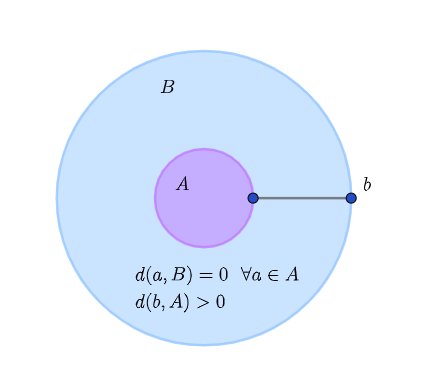
\includegraphics[scale = 0.4]{img/C4/no-distancia-hausdorff.png}
    \caption{Contraejemplo a la distancia entre conjuntos}
        \label{fig:contraejemplo-distancia}
\end{figure}

\begin{definicion}
    Dado un espacio de Banach $(X,d)$, en el espacio de fractales $\mathcal{H}(X)$ Se define la \textbf{distancia de Hausdorff} o \textbf{métrica de Hausdorff} como:
    $$
    h(d)(A,B)=\max\{d(A,B),d(B,A)\} \ \ \forall A,B\in\mathcal H(X).
    $$
\end{definicion}

En adelante denotaremos únicamente $h(\cdot,\cdot)$, omitiendo la dependencia de la distancia del espacio original.

Podemos comprobar en \cite{Barnsley}[Sección 2.6] que, en efecto, $h$ es una distancia. Además, en \cite{Barnsley}[Sección 2.7] se prueba que el espacio métrico $(\mathcal{H}(X), h(d))$ es completo.



